\section{The constant \texorpdfstring{$A(p)$}{A(p)}}
\label{sec:Ap}

Everything in \cref{sec:qsd} reduced to the single constant
\begin{equation}
\label{eq:Ap-def}
A(p) = \lim_{n\to\infty}\frac{S_n}{(2p)^n},\qquad p\in[0,\tfrac12),
\end{equation}
whose reciprocal is the quasi-stationary mean. Approximate values are obtained by iterating \(S_{n+1}=f(S_n)\) until near stationarity and forming \(S_n/(2p)^n\). Over most of the interval this is reliable; it fails as \(p\to\tfrac12^-\), because the number of generations needed grows without bound.

No formula in elementary functions is known for \(A(p)\). This section records what is known: an exact infinite product (\cref{sec:product}); an exact series with two-sided bounds that pin \(A(p)\) between the continuous-time constant of \cref{sec:cts} and twice that bound's companion (\cref{sec:Abounds}); the near-critical asymptotic \(A(p)\sim2(1-2p)\) (\cref{sec:asymptotic}); a resolution of the discrete--continuous discrepancy (\cref{sec:compare}); an account of symbolic-regression searches (\cref{sec:GA}); and the dynamical argument explaining why a closed form is not to be expected (\cref{sec:koenigs}). \Cref{sec:practical} summarises practical computation.

\subsection{An infinite-product representation}
\label{sec:product}

Start from the survival map \(S_{n+1}=2pS_n-pS_n^2\), \(S_0=1\), and set \(S_n=2w_n\). Then
\begin{equation}
\label{eq:logistic}
w_{n+1} = 2p\,w_n(1-w_n) = r\,w_n(1-w_n),\qquad r = 2p,\ \ w_0 = \tfrac12 ,
\end{equation}
which is the logistic map. The celebrated period-doubling cascade as \(r\) increases from \(0\) to \(4\) is recalled in \cref{fig:period_double}; the subcritical branching window is \(r\in[0,1)\), at the extreme left of that picture, where the origin is globally attracting. That this corner of the logistic family is nevertheless enough to obstruct a closed form is the content of \cref{sec:koenigs}.

\begin{figure}[ht]
    \centering
    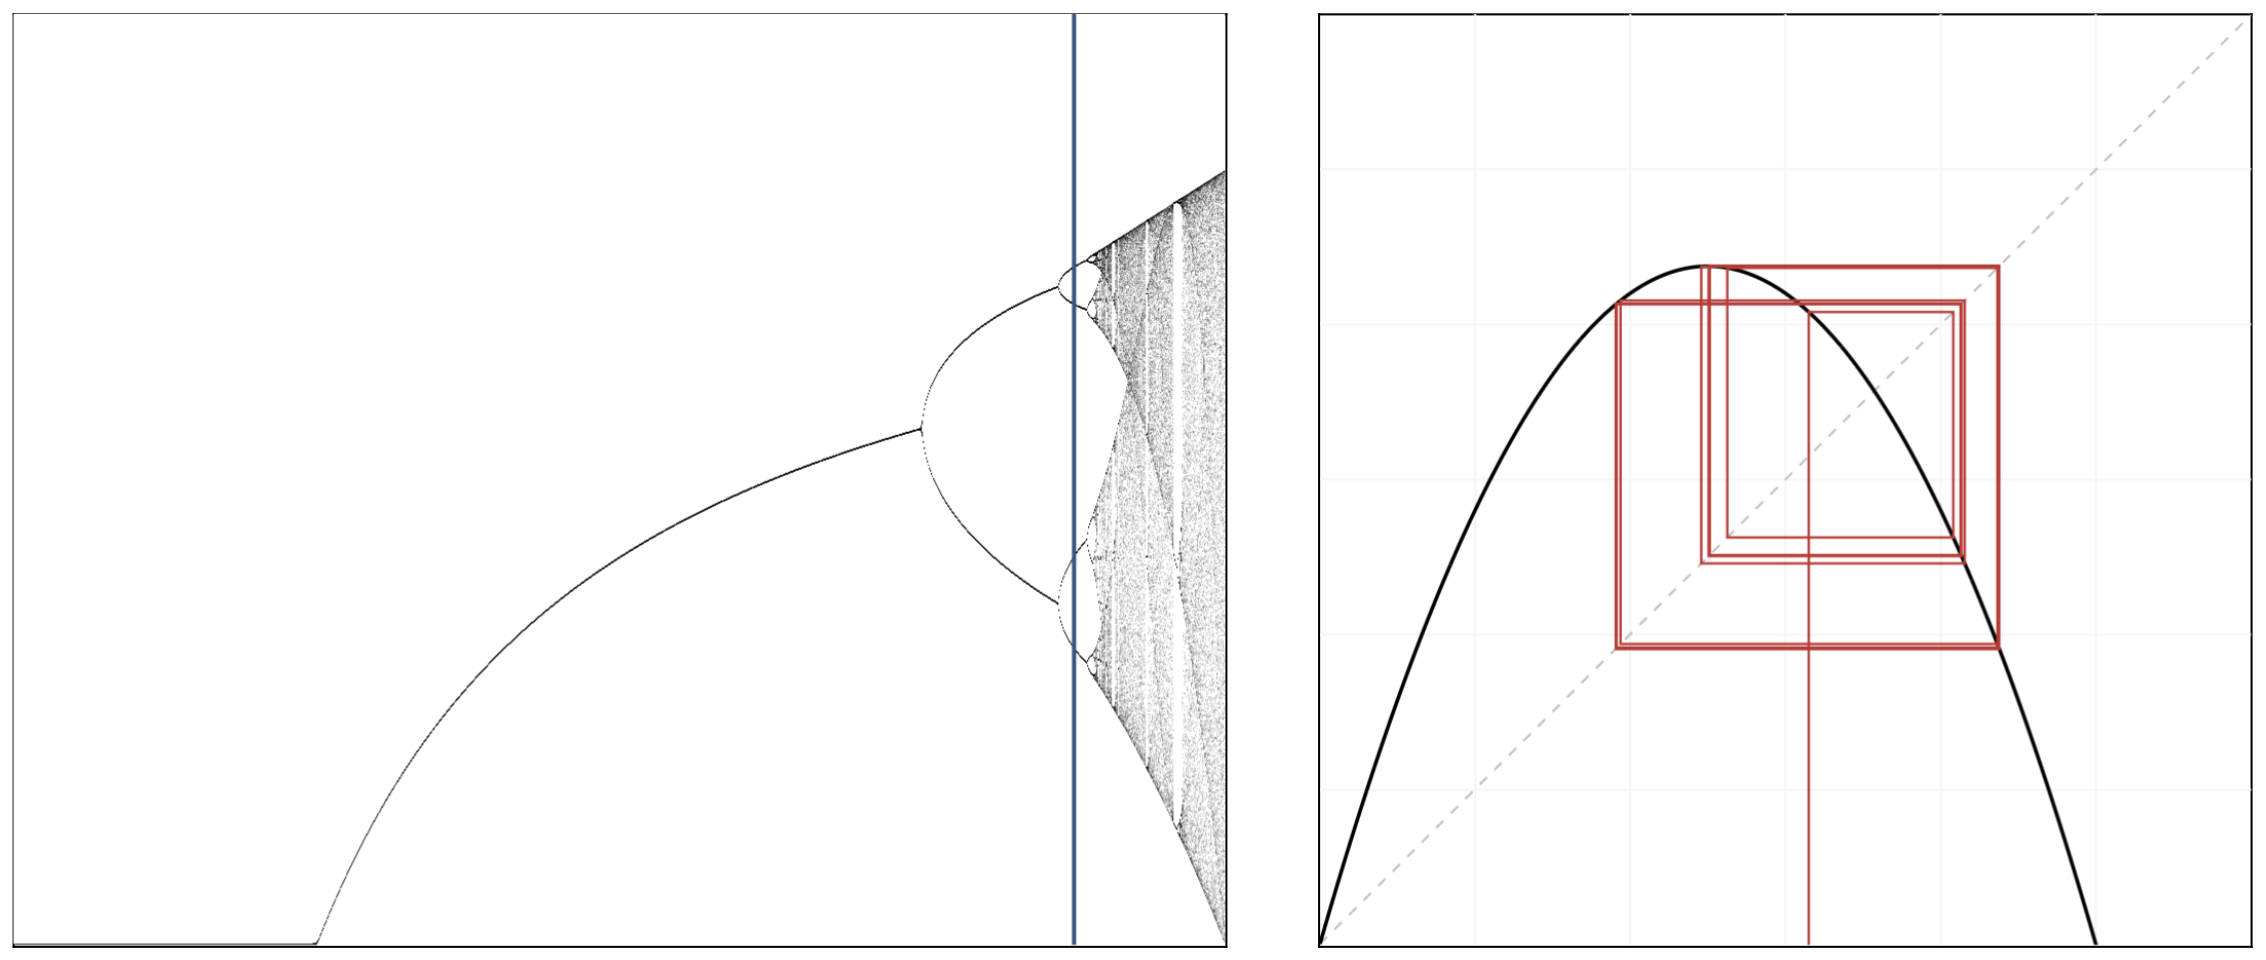
\includegraphics[width=0.86\textwidth]{figures/IMG_ch3/period_double.png}
    \caption{Bifurcation diagram of the logistic map \(w\mapsto rw(1-w)\). The regime relevant to subcritical branching is \(r=2p\in[0,1)\), off the left-hand edge, where the dynamics are as simple as they can be.}
    \label{fig:period_double}
\end{figure}

In terms of \(w\),
\begin{equation}
\label{eq:Aw}
A(p) = 2\lim_{n\to\infty}\frac{w_n}{r^n}.
\end{equation}
Any sequence admits a telescoping product representation. Applying it to \(x_n=w_n/r^n\) yields ratios
\begin{equation*}
\frac{x_{k+1}}{x_k}=1-w_k,
\end{equation*}
and therefore
\begin{equation}
\label{eq:prodFormula}
A(p) = \frac12\prod_{k=1}^{\infty}\lrb{1-w_k} = \frac12\prod_{k=1}^{\infty}\lrb{1-\frac{S_k}{2}}.
\end{equation}

\subsubsection*{Convergence}

For \(0<w_k<1\) the product \(\prod_{k\ge1}(1-w_k)\) converges to a strictly positive limit if and only if \(\sum w_k<\infty\). From \cref{eq:logistic} with \(0<r<1\) one has \(w_{n+1}<rw_n\), so \(w_n\le w_0 r^n\). The bound is summable, the product converges, and the limit \cref{eq:Ap-def} exists in \((0,\tfrac12)\) for \(p\in(0,\tfrac12)\).

\subsubsection*{Is this an advance?}

Only a modest one. Partial products of \cref{eq:prodFormula} are monotone decreasing and supply rigorous upper bounds on \(A(p)\), which the raw ratio \(S_n/(2p)^n\) does not. Computing the factors still requires iterating the nonlinear map, so the near-critical difficulty remains. The product does, however, open a route to the sharper series of the next subsection.

\subsection{An exact series and two-sided bounds}
\label{sec:Abounds}

Write \(r=2p\) and \(S_{n+1}=rS_n\bigl(1-S_n/2\bigr)\). Define \(v_n=r^n/S_n\), so that \(v_n\to1/A(p)\). Then
\begin{equation*}
v_{n+1}-v_n = \frac{r^n}{2-S_n}.
\end{equation*}
Summing from \(v_0=1\) yields an exact representation of the quasi-stationary mean.

\begin{proposition}[Series representation]
\label{prop:series}
For \(p\in[0,\tfrac12)\), with \(S_n\) generated by \cref{SnIter},
\begin{equation}
\label{eq:Aseries}
\frac{1}{A(p)} = 1 + \sum_{n=0}^{\infty}\frac{(2p)^n}{2-S_n}.
\end{equation}
\end{proposition}

Unlike the product, this form isolates geometric decay in a factor independent of the early nonlinear dynamics; the whole of the nonlinearity sits in the bounded denominator \(2-S_n\in[1,2)\). Bounding the denominator by its extremes and summing the resulting geometric series produces the following.

\begin{proposition}[Two-sided bounds]
\label{prop:bounds}
Write \(\varepsilon = 1-2p\). Then for \(p\in(0,\tfrac12)\)
\begin{equation}
\label{eq:Abounds}
\frac{\varepsilon}{1+\varepsilon} \;<\; A(p) \;<\; \frac{2\varepsilon}{1+2\varepsilon},
\end{equation}
equivalently
\begin{equation}
\label{eq:Aboundsexplicit}
\frac{1-2p}{2(1-p)} \;<\; A(p) \;<\; \frac{2(1-2p)}{3-4p}.
\end{equation}
The lower bound is exactly half the continuous-time constant of \cref{eq:Acts}:
\begin{equation}
\label{eq:halfAc}
A(p) > \tfrac12 A_{\text{c}}(p).
\end{equation}
\end{proposition}

\begin{proof}
Since \(0<S_n\le1\), one has \(\tfrac12 r^n < r^n/(2-S_n)\le r^n\) (equality on the right only at \(n=0\)). Summing and using \(\sum r^n=1/\varepsilon\) gives
\begin{equation*}
1+\frac{1}{2\varepsilon} \;<\; \frac{1}{A(p)} \;<\; 1+\frac{1}{\varepsilon},
\end{equation*}
and inversion produces \cref{eq:Abounds}. Substituting \(\varepsilon=1-2p\) gives \cref{eq:Aboundsexplicit}, whose lower bound equals \(\tfrac12 A_{\text{c}}(p)\).
\end{proof}

As \(p\to0\), \(\varepsilon\to1\) and the lower bound tends to \(\tfrac12\). Combined with the parity bound below, \(A(0^+)=\tfrac12\). As \(p\to\tfrac12^-\), the lower bound behaves like \(\varepsilon\) and the upper like \(2\varepsilon\); \cref{sec:asymptotic} shows that the upper bound is attained asymptotically. Thus \(A(p)\) runs from its lower bound at one end of the interval to its upper bound at the other, and no constant rescaling of \(A_{\text{c}}\) can reproduce it.

\begin{proposition}[Parity bound]
\label{prop:parity}
For the binary Galton--Watson process started from a single individual, \(A(p)\le\tfrac12\) for all \(p\in[0,\tfrac12)\), with equality approached as \(p\to0\).
\end{proposition}

\begin{proof}
Every individual leaves \(0\) or \(2\) offspring, so \(\zz_n\) is even for every \(n\ge1\). Conditional on survival, \(\zz_n\ge2\), hence \(\mean{\zz_n\mid \zz_n>0}\ge2\). Taking \(n\to\infty\) and using \cref{eq:qsmean} gives \(1/A(p)\ge2\). As \(p\to0\) the conditional population is \(2\) with probability tending to one, so the bound is attained in the limit.
\end{proof}

\begin{table}[ht]
\centering
\caption{The constant \(A(p)\) from the product \cref{eq:prodFormula} in high-precision arithmetic, against the bounds of \cref{prop:bounds} and the near-critical asymptotic \(2(1-2p)\). The last two columns give the quasi-stationary mean and the number of factors needed for full precision.}
\label{tab:Avals}
\begin{tabular}{ccccccr}
\toprule
$p$ & $\tfrac12 A_{\text{c}}(p)$ & $A(p)$ & $\dfrac{2(1-2p)}{3-4p}$ & $2(1-2p)$ & $1/A(p)$ & iterations\\
\midrule
0.05   & 0.473684 & 0.486180 & 0.642857 & 1.800000 & 2.0568 & 45 \\
0.1    & 0.444444 & 0.469382 & 0.615385 & 1.600000 & 2.1305 & 64 \\
0.2    & 0.375000 & 0.423895 & 0.545455 & 1.200000 & 2.3591 & 113 \\
0.3    & 0.285714 & 0.353967 & 0.444444 & 0.800000 & 2.8251 & 201 \\
0.4    & 0.166667 & 0.237647 & 0.285714 & 0.400000 & 4.2079 & 458 \\
0.45   & 0.090909 & 0.145069 & 0.166667 & 0.200000 & 6.8933 & 966 \\
0.48   & 0.038462 & 0.068011 & 0.074074 & 0.080000 & 14.7036 & 2\,473 \\
0.49   & 0.019608 & 0.036395 & 0.038462 & 0.040000 & 27.4764 & 4\,965 \\
0.499  & 0.001996 & 0.003944 & 0.003984 & 0.004000 & 253.519 & 48\,992 \\
0.4999 & 0.000200 & 0.000399 & 0.000400 & 0.000400 & 2504.65 & 478\,905 \\
\bottomrule
\end{tabular}
\end{table}

\subsection{Behaviour as \texorpdfstring{$p\to\tfrac12^-$}{p to 1/2}}
\label{sec:asymptotic}

The series \cref{eq:Aseries} delivers the near-critical asymptotic transparently. Fix \(\varepsilon=1-2p\) small. The summand \(r^n/(2-S_n)\) involves two scales: geometric decay on \(n\sim1/\varepsilon\), and survival \(S_n\) already near its critical law \(S_n\sim2/n\) over that range. For the overwhelming majority of weighted terms, \(S_n\approx0\) and the summand is \(\approx r^n/2\). Summing,
\begin{equation*}
\sum_{n=0}^{\infty}\frac{r^n}{2-S_n} \;\approx\; \frac{1}{2\varepsilon},
\end{equation*}
so \(1/A(p)\sim1/(2\varepsilon)\) and
\begin{equation}
\label{eq:Aasym}
\boxed{\;A(p) \sim 2\varepsilon = 2(1-2p)\qquad\text{as } p\to\tfrac12^-.\;}
\end{equation}
Equivalently, the quasi-stationary mean diverges like the reciprocal of the distance from criticality. In particular \(A(p)\) meets the axis at \(p=\tfrac12\) with gradient \(-4\), a diagnostic used repeatedly below.

The continuum equation of \cref{sec:riccati} recovers the same leading asymptotic after matching to \(S_n\sim2/n\); the series argument avoids the delicate second matching step.

\begin{remark}[Rate of approach]
\label{rem:rate}
Numerically, \(A(p)/2\varepsilon\) approaches \(1\) slowly: high-precision evaluation of \cref{eq:prodFormula} gives \(A/2\varepsilon = 0.90987\), \(0.98612\), \(0.99814\), \(0.99977\) and \(0.999972\) at \(\varepsilon = 2\times10^{-2}\) down to \(2\times10^{-6}\). Fitting the deficit suggests
\begin{equation*}
A(p) = 2\varepsilon\Bigl[1+O\bigl(\varepsilon\ln(1/\varepsilon)\bigr)\Bigr].
\end{equation*}
The logarithmic correction limits the practical usefulness of \cref{eq:Aasym} except very near criticality.
\end{remark}

\subsection{Why the discrete and continuous constants differ}
\label{sec:compare}

The two constants are
\begin{equation*}
A_{\text{c}}(p) = \frac{1-2p}{1-p}
\qquad\text{(continuous time)},
\qquad
A(p) = \lim_{n\to\infty}\frac{S_n}{(2p)^n}
\qquad\text{(discrete time)}.
\end{equation*}
\Cref{prop:bounds} shows that \(A>\tfrac12 A_{\text{c}}\) strictly, with equality only in the limit \(p\to0\). Combining with \cref{eq:Aasym,eq:Acts},
\begin{equation}
\label{eq:ratiolimits}
\frac{A(p)}{A_{\text{c}}(p)} \;\longrightarrow\; \tfrac12 \ \ (p\to0),
\qquad
\frac{A(p)}{A_{\text{c}}(p)} \;\longrightarrow\; 1 \ \ (p\to\tfrac12^-),
\end{equation}
with intermediate values \(0.503\), \(0.528\), \(0.619\), \(0.798\), \(0.928\) and \(0.988\) at
\(p = 0.01\), \(0.1\), \(0.3\), \(0.45\), \(0.49\), and \(0.499\).
No constant factor reconciles the curves.

At \(p\to0\) the factor of two is a counting effect: binary discrete survivors are always even (\cref{prop:parity}), and deep subcritical conditioning on survival means conditioning on a population of exactly two, so the quasi-stationary mean is \(2\). In continuous time a survivor is a single individual that has not yet died, so the mean is \(1\). Near \(p\to\tfrac12^-\) both constants share the universal \(2\varepsilon\) critical scaling, and discreteness of the generational clock ceases to matter to leading order.

\subsection{Searching for a closed form}
\label{sec:GA}

Before the Koenigs connection was appreciated, several methods were tried in the hope of an elementary formula for \(A(p)\).

The continuum route of \cref{sec:riccati} determines the shape of the decay but leaves the integration constant --- that is, \(A(p)\) --- undetermined.

Symbolic regression by genetic algorithm was also attempted: generate candidate functions, retain those that best match high-precision numerical \(A(p)\), vary and reselect over many cycles \cite{stanley2002evolving,cohen2024physics}. Polynomial genomes, rational-coefficient polynomials, and ratios of polynomials all produced visually excellent fits that failed basic diagnostics. A representative rational candidate,
\begin{equation}
\label{eq:A1hat}
\hat A_1(p) = \frac{\tfrac12(1-2p)(1+2p)}{1 + \tfrac12 p - \tfrac52 p^2 - \tfrac65 p^3 + \tfrac65 p^4},
\end{equation}
passes through \((0,\tfrac12)\) and \((\tfrac12,0)\) but arrives at criticality with gradient \(-3.636\) rather than \(-4\). Nested elementary expressions from tree search performed similarly; two arbitrary examples are
\begin{multline}
\label{eq:A2hat}
\hat A_2(p) = 0.31696448624690005\,
\ln\!\Biggl(\Biggl|\cos\!\biggl(\left(\frac{1}{3.19801133824532}\right)^{\!1/4}\\
+\, p\biggl[\sin\!\Bigl(\cos\!\bigl(|p|\,(0.621865696665606 - p)\,\cos(\ee^{\ee^{p}})\bigr)\Bigr) + |p|\biggr]\biggr)\Biggr|\Biggr)
+ 0.5982282661889831
\end{multline}
and
\begin{equation}
\label{eq:A3hat}
\hat A_3(p) = \frac{-0.616647881739505\,\ee^{-0.552605335919693\,\ee^{p}}}{\sin(\cos p) - |p|} + 0.921964323679771 .
\end{equation}

\begin{figure}[ht]
\centering
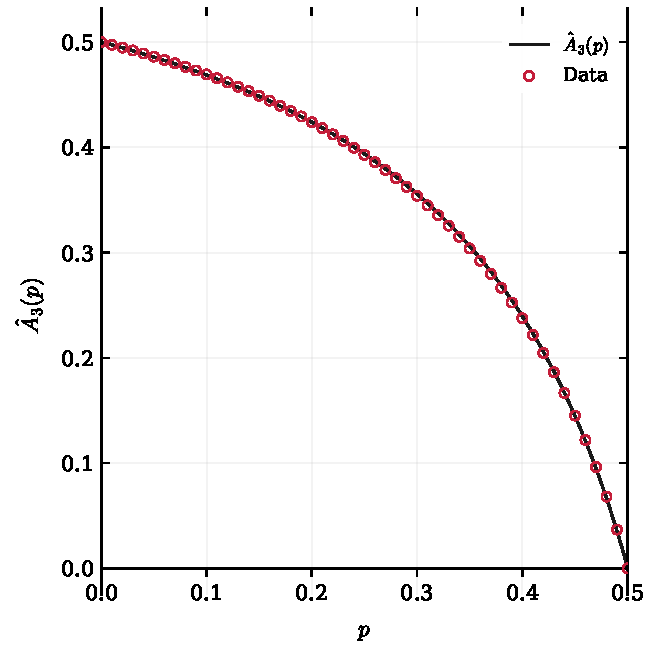
\includegraphics[width=0.56\textwidth]{figures/IMG_ch3/A3_hat_plot.pdf}
\caption{Symbolic-regression candidate \(\hat A_3(p)\) of \cref{eq:A3hat} (solid) against numerical \(A(p)\) (red circles). Visual agreement is excellent; \(\hat A_3(\tfrac12)=9.1\times10^{-4}\) rather than \(0\), and the critical gradient is \(-3.63\) rather than \(-4\). Errors of this size devastate \(1/A\) near criticality.}
\label{fig:A3hat}
\end{figure}

The recurring defect is failure to hit \((\tfrac12,0)\) with gradient \(-4\). As \(A\to0\), an absolute error that vanishes on a plot of \(A\) produces an \(O(1)\) and eventually unbounded error in the quasi-stationary mean \(1/A\).

A pragmatic splice of a fitted curve onto the asymptotic, for example
\begin{equation}
\label{eq:A4hat}
\hat A_4(p) =
\begin{cases}
-0.04011483983619545\,\ee^{\ee^{2p}} + 0.6079994336528085, & p < 0.499962,\\[2mm]
2-4p, & p \ge 0.499962,
\end{cases}
\end{equation}
works numerically, but if one is to splice it is better to splice onto something exact; \cref{sec:practical} does so. The deeper lesson is that curve-fitting cannot distinguish a function with a closed form from one without: many radically different expressions track \(A(p)\) closely on a bounded interval.

\subsection{The Koenigs connection}
\label{sec:koenigs}

A dynamical argument explains why no elementary closed form should be expected: \(A(p)\) is a value of the Koenigs linearising function of the logistic map, and that function is non-elementary throughout the parameter range of interest.

\begin{definition}[Koenigs function]
\label{def:koenigs}
Let \(f(z) = rz(1-z)\) have a fixed point at \(z=0\) with multiplier \(r = f'(0)\), and suppose \(|r|\notin\{0,1\}\). Koenigs \cite{Koenigs1884} proved that there exists a unique function \(\psi_r\), analytic near the origin, satisfying the Schr\"oder equation
\begin{equation}
\label{eq:schroder}
\psi_r\bigl(f(z)\bigr) = r\,\psi_r(z),
\qquad
\psi_r(0)=0,
\qquad
\psi_r'(0)=1 .
\end{equation}
\end{definition}

The Koenigs function is a change of coordinate that straightens the dynamics: in the \(\psi\) coordinate the nonlinear map \(f\) becomes multiplication by \(r\) (\cref{fig:koenigs}). Here \(f(z)=rz(1-z)\) is exactly \cref{eq:logistic}, with multiplier \(r=2p\in(0,1)\).

\begin{figure}[ht]
\centering
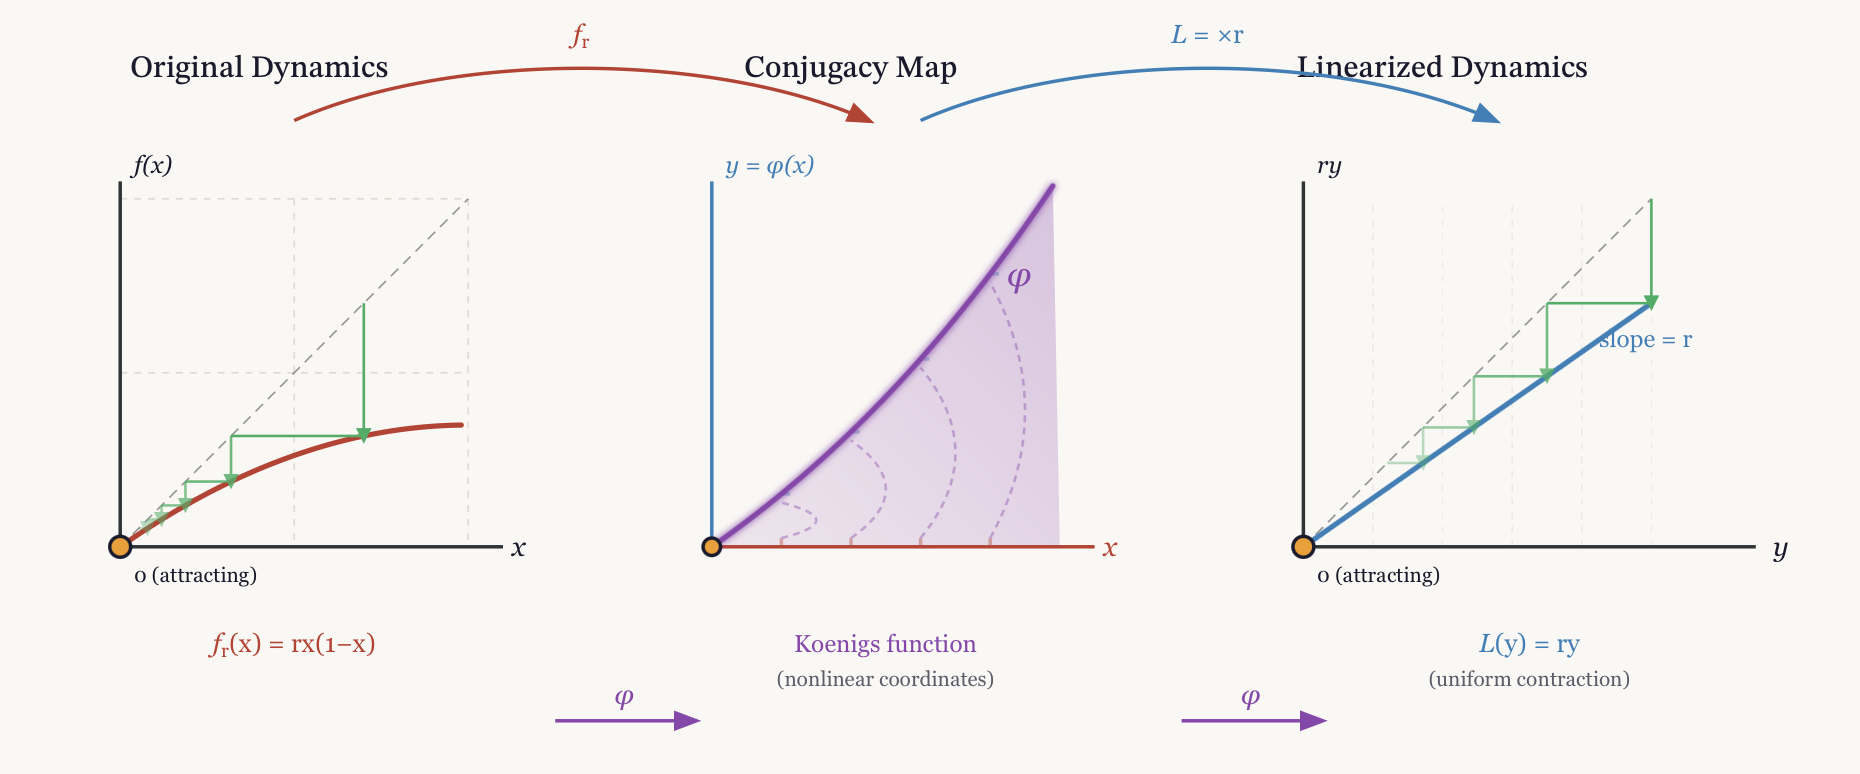
\includegraphics[width=0.72\textwidth]{figures/IMG_ch3/figure2_koenigs_linearization.png}
\caption{Koenigs linearisation of the logistic map near an attracting fixed point: \(\psi_r(f_r(x))=r\psi_r(x)\).}
\label{fig:koenigs}
\end{figure}

\begin{proposition}
\label{prop:AisKoenigs}
For \(p\in(0,\tfrac12)\) and \(r=2p\),
\begin{equation}
\label{eq:AeqKoenigs}
A(p) = 2\,\psi_r\!\lrb{\tfrac12}.
\end{equation}
\end{proposition}

\begin{proof}
Iterating \cref{eq:schroder} along the orbit \(w_n\) of \cref{eq:logistic} gives \(\psi(w_0)=\psi(w_n)/r^n\) for every \(n\). Passing to the limit and using \(\psi(z)/z\to1\) as \(z\to0\) with \(w_n\to0\) yields \(\psi(w_0)=\lim_n w_n/r^n\). Comparing with \cref{eq:Aw} and \(w_0=\tfrac12\) gives \(A(p)=2\psi_r(\tfrac12)\).
\end{proof}

\subsubsection*{When is \texorpdfstring{$\psi_r$}{psi} elementary?}

Essentially never. The logistic family is affinely conjugate to the quadratic family \(P_c(z)=z^2+c\); substituting \(x=-z/r+\tfrac12\) in \(f_r\) gives \(P_c\) with
\begin{equation}
\label{eq:cofr}
c = \frac{2r-r^2}{4}.
\end{equation}
Under this correspondence, \(r\in(0,1)\) maps to \(c\in(0,\tfrac14)\) (\cref{fig:conjugacy}). Becker and Bergweiler \cite{Becker1995} proved that for a rational map of degree at least two with fixed-point multiplier \(\lambda\), \(0<|\lambda|<1\), the associated Koenigs linearisation satisfies an algebraic differential equation only when the map is analytically conjugate to a monomial \(z\mapsto z^{\pm d}\) or a Chebyshev polynomial \(\pm T_d\). For the quadratic family the exceptional cases are \(c=0\) and \(c=-2\), corresponding to \(r=2\) and \(r=4\).

Every elementary function in the Liouville sense satisfies an algebraic differential equation. A hypertranscendental function satisfies none. Since
\begin{equation*}
\lrb{0,\tfrac14}\cap\{0,-2\} = \emptyset,
\end{equation*}
no \(r\) in the branching window is exceptional: for each fixed \(r\in(0,1)\), \(\psi_r\) is hypertranscendental and in particular not elementary.

\begin{figure}[ht]
\centering
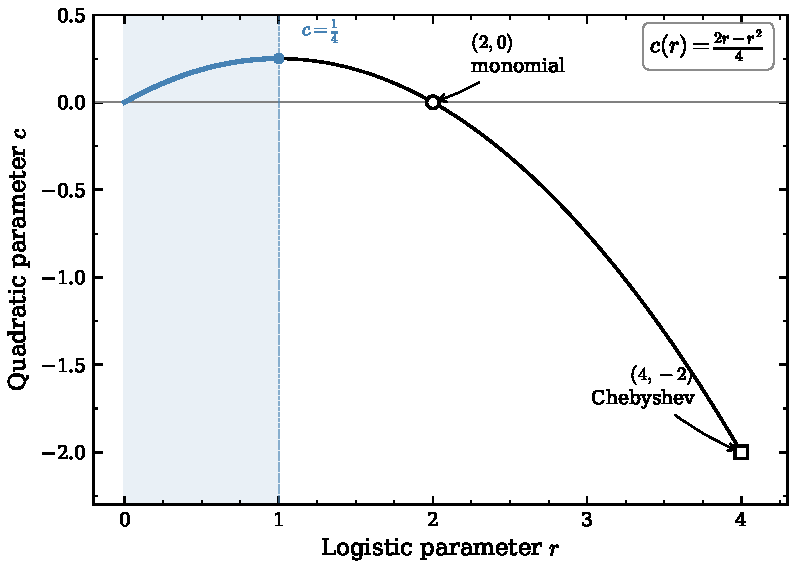
\includegraphics[width=0.66\textwidth]{figures/IMG_ch3/figure1_parameter_conjugacy.pdf}
\caption{Parameter correspondence \(c(r)=(2r-r^2)/4\) between the logistic and quadratic families. The shaded segment \(r\in(0,1)\) maps to \(c\in(0,\tfrac14)\). The integrable parameters \(r=2\) (\(c=0\)) and \(r=4\) (\(c=-2\)) lie outside it.}
\label{fig:conjugacy}
\end{figure}

\paragraph{The monomial case, \(r=2\).}
Here \(f_2(x)=2x(1-x)\). The substitution \(u=1-2x\) gives \(u\mapsto u^2\), linearised by the logarithm. Returning to \(x\) and imposing the Koenigs normalisation,
\begin{equation}
\label{eq:psi2}
\psi_2(x) = -\tfrac12\ln(1-2x).
\end{equation}

\paragraph{The Chebyshev case, \(r=4\).}
Here \(f_4(x)=4x(1-x)\) is conjugate to angle doubling via \(x=\sin^2\theta\), and
\begin{equation}
\label{eq:psi4}
\psi_4(x) = \bigl(\arcsin\sqrt{x}\,\bigr)^2 .
\end{equation}

\begin{remark}[Attracting versus repelling]
\label{rem:attractrepel}
At \(r=2\) and \(r=4\) the multiplier satisfies \(|r|>1\), so the origin is repelling. The functions \cref{eq:psi2,eq:psi4} are Poincar\'e-type linearisations rather than attracting-Koenigs maps, and neither parameter lies in \(r=2p\in[0,1)\). They illustrate solvable cases; they do not bear on \(A(p)\).
\end{remark}

\subsubsection*{What this does and does not establish}

For each fixed \(r\in(0,1)\), \(z\mapsto\psi_r(z)\) is hypertranscendental. Combined with \cref{prop:AisKoenigs}, \(A(p)\) is a value of a non-elementary function at \(z=\tfrac12\). This strongly indicates that the searches of \cref{sec:GA} were doomed.

What is \emph{not} established is that the map \(p\mapsto A(p)\) admits no elementary description: hypertranscendence of \(\psi_r\) in its argument is logically distinct from transcendence of the values \(2\psi_{2p}(\tfrac12)\). No rigorous negative result for \(p\mapsto A(p)\) is claimed. The honest summary is that no closed form is known, that the structural reason for expecting none is the one just given, and that the numerical evidence is consistent with there being none.

Under \(c=\lambda/2-\lambda^2/4\), the branching window \(r\in(0,1)\) is the real diameter of the main cardioid of the Mandelbrot set, from the centre \(c=0\) out to the parabolic cusp \(c=\tfrac14\) (criticality). \Cref{fig:mandelbrot} places the segment in context. Throughout the window the Julia set is a quasicircle bounding the basin of the attracting fixed point, and the Koenigs function is the conformal coordinate that linearises the dynamics inside that basin. A function whose natural domain has no smooth description is a poor candidate for a closed form; \(A(p)\), being one of its values, inherits the difficulty.

\begin{figure}[ht]
\centering
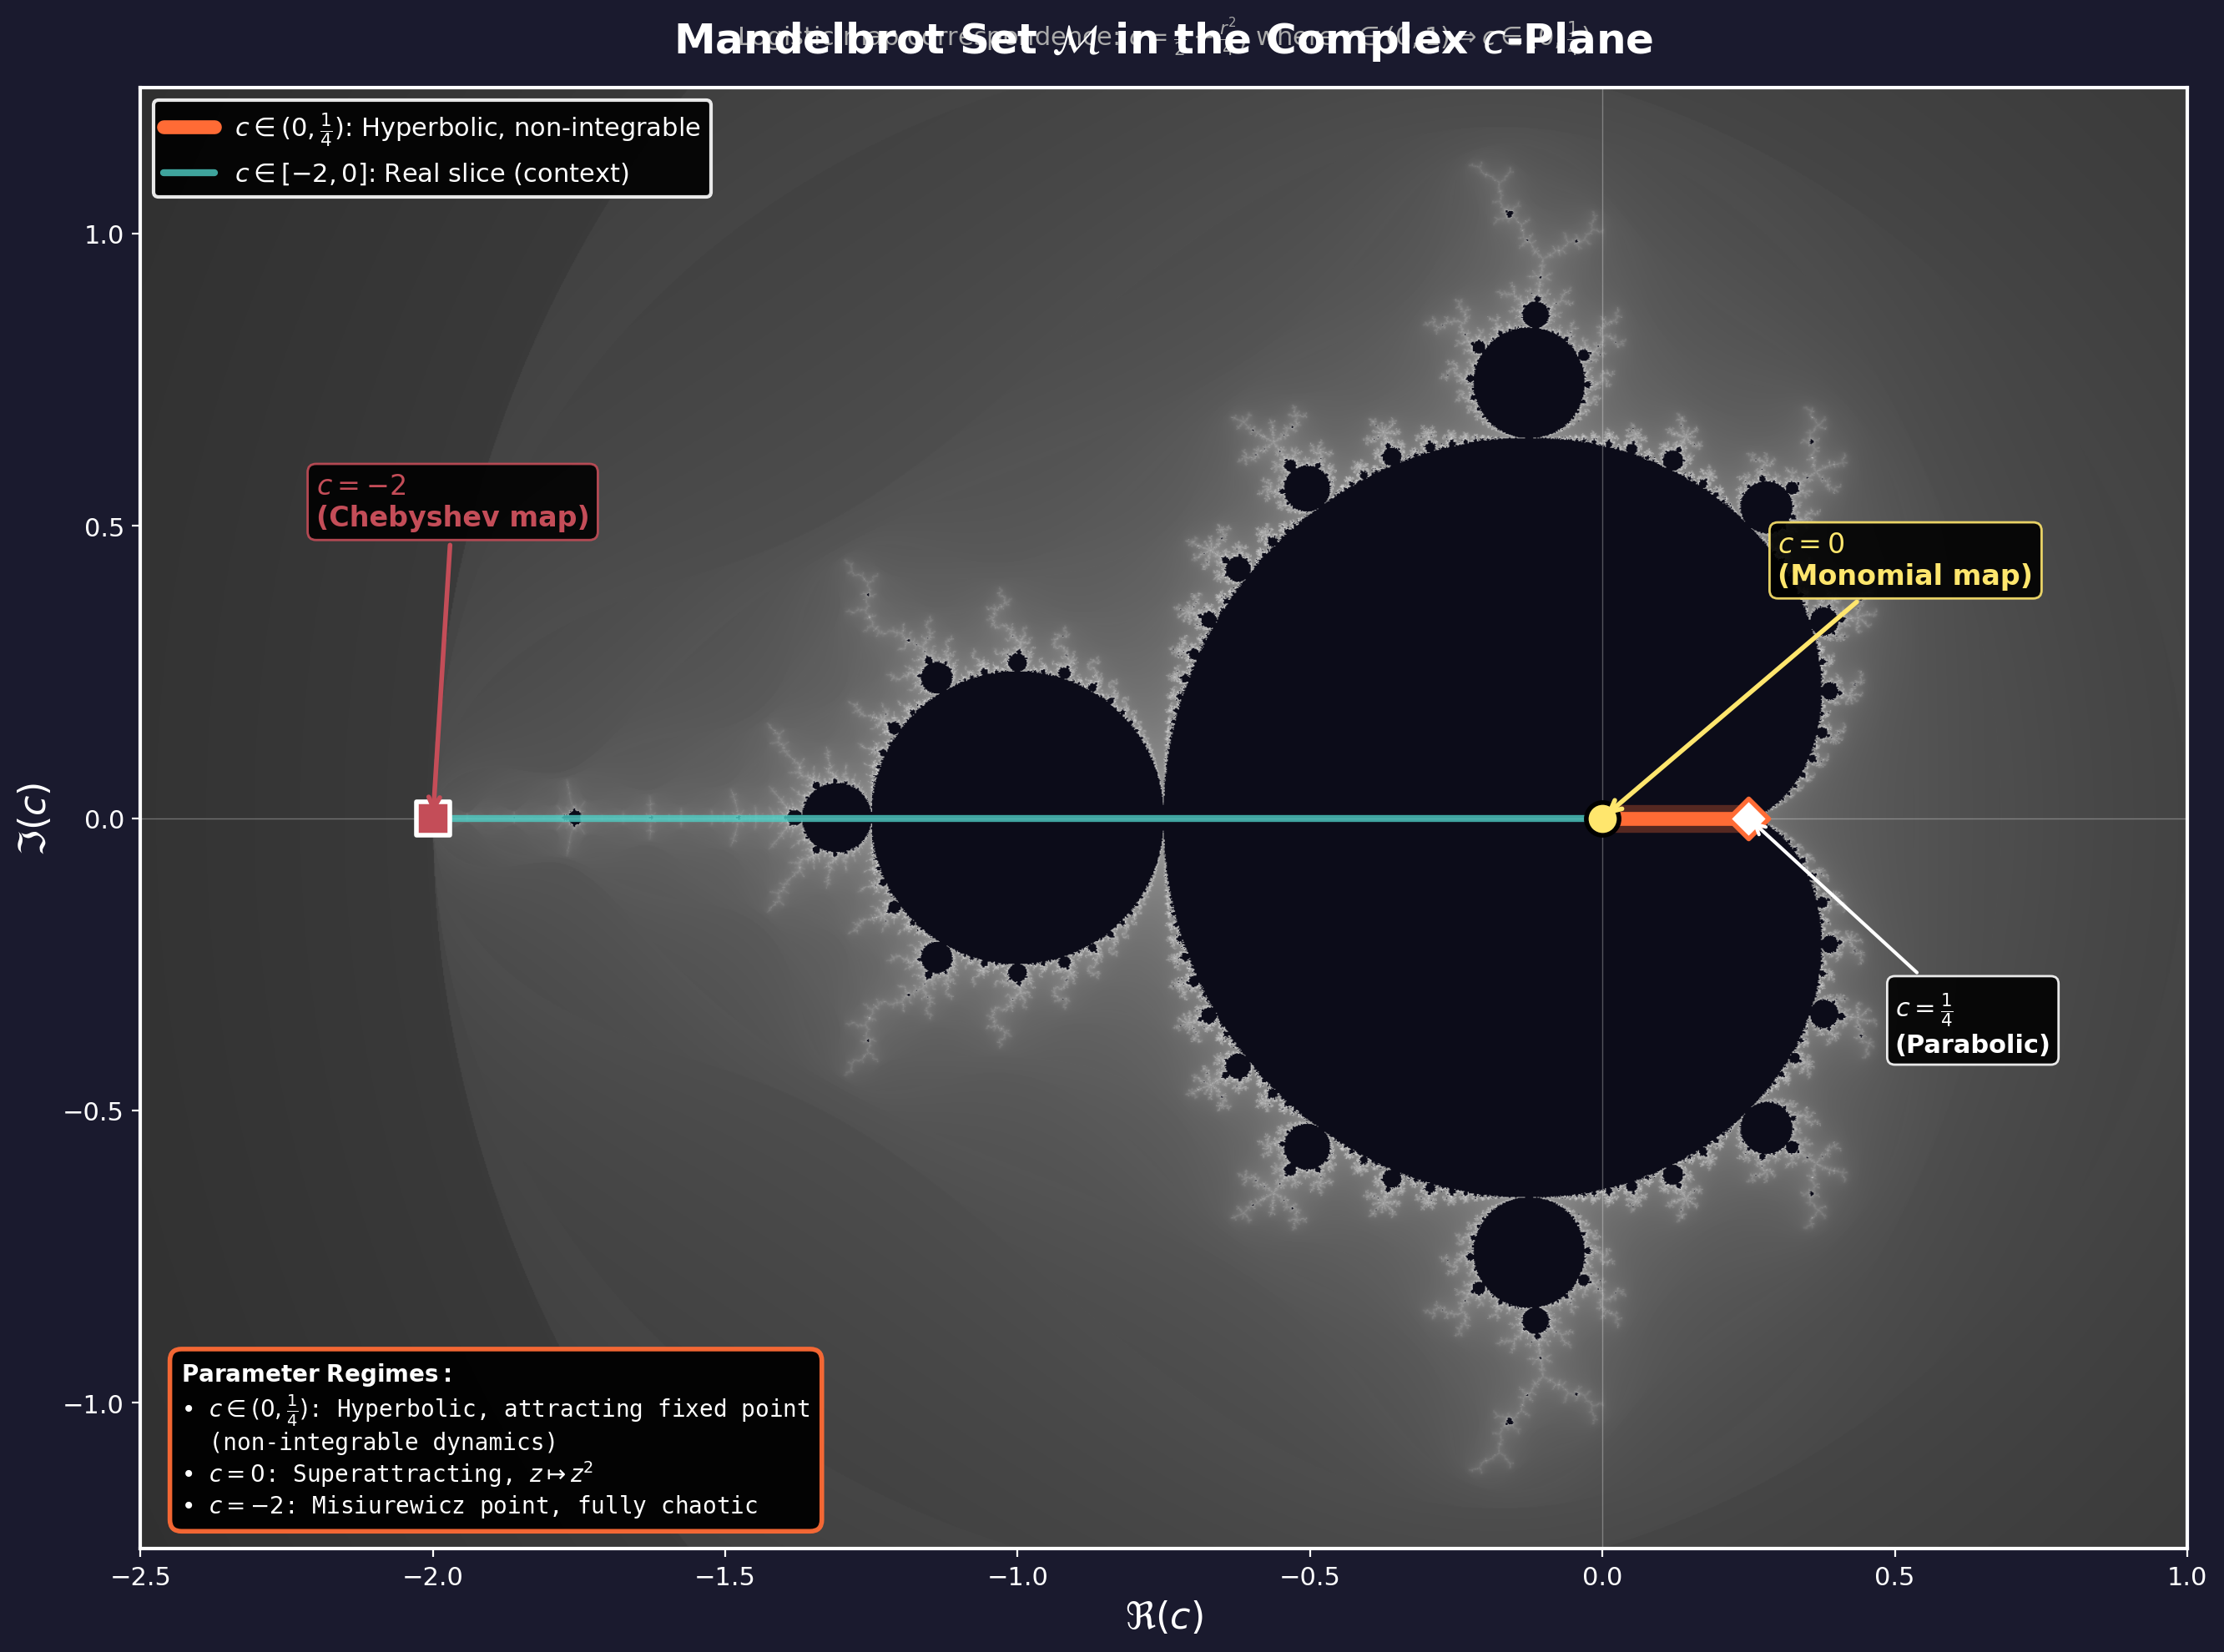
\includegraphics[width=0.92\textwidth]{figures/IMG_ch3/figure4_mandelbrot_context.png}
\caption{The Mandelbrot set with the interval \(c\in(0,\tfrac14)\) highlighted --- the image of the subcritical branching window under \(c=(2r-r^2)/4\). Integrable parameters \(c=0\) and \(c=-2\) are marked.}
\label{fig:mandelbrot}
\end{figure}

\subsection{Computing \texorpdfstring{$A(p)$}{A(p)} in practice}
\label{sec:practical}

In the absence of an exact formula one approximates, splitting the interval into regimes suggested by \cref{sec:Abounds}.

Over most of the range, the infinite product \cref{eq:prodFormula} converges quickly and partial products bound \(A(p)\) from above. Difficulty is confined to a neighbourhood of \(p=\tfrac12\): as \(A\to0\), absolute errors in \(A\) become unbounded errors in \(1/A\); and as criticality is approached, \(S_n\) recedes to zero ever more slowly. \Cref{tab:Avals} records the cost: of order \(10^2\) iterations at \(p=0.2\), \(10^3\) at \(p=0.45\), and nearly \(5\times10^5\) at \(p=0.4999\).

The remedy is to hand the near-critical region to the asymptotic \cref{eq:Aasym}:
\begin{equation}
\label{eq:Apractical}
A(p) \approx
\begin{cases}
\displaystyle \frac12\prod_{k=1}^{N}\lrb{1-\frac{S_k}{2}}, & p<c,\quad N\gg1,\\[14pt]
2-4p, & p\ge c,
\end{cases}
\end{equation}
with crossover \(c\) just below \(\tfrac12\). At \(c=0.4999\) (\(\varepsilon=2\times10^{-4}\)) the relative error of the asymptotic is of order a few parts in \(10^3\), while the product still converges in a few hundred thousand iterations. Any \(c\) in \(0.499\)--\(0.4999\) yields accuracy better than one per cent throughout. This is the recipe underlying the numerical values quoted in this chapter, including those in \cref{fig:condmean,tab:Avals}.

\FloatBarrier
